\documentclass[12pt]{article}
 
\usepackage[margin=1in]{geometry} 
\usepackage{amsmath,amsthm,amssymb}
\usepackage{enumerate}
\usepackage{graphicx}
\usepackage{hyperref}
\usepackage{xcolor}
\usepackage{float}

\usepackage{epstopdf}
\epstopdfDeclareGraphicsRule{.tif}{png}{.png}{convert #1 \OutputFile}
\AppendGraphicsExtensions{.tif}

\graphicspath{ {/home/taylor/repos/visual/img/} }
 
\newcommand{\N}{\mathbb{N}}
\newcommand{\Z}{\mathbb{Z}}
 
\newenvironment{theorem}[2][Theorem]{\begin{trivlist}
\item[\hskip \labelsep{\bfseries #1}\hskip \labelsep{\bfseries #2.}]}{\end{trivlist}}
\newenvironment{lemma}[2][Lemma]{\begin{trivlist}
\item[\hskip \labelsep{\bfseries #1}\hskip \labelsep{\bfseries #2.}]}{\end{trivlist}}
\newenvironment{exercise}[2][Exercise]{\begin{trivlist}
\item[\hskip \labelsep{\bfseries #1}\hskip \labelsep{\bfseries #2.}]}{\end{trivlist}}
\newenvironment{problem}[2][Problem]{\begin{trivlist}
\item[\hskip \labelsep{\bfseries #1}\hskip \labelsep{\bfseries #2.}]}{\end{trivlist}}
\newenvironment{question}[2][Question]{\begin{trivlist}
\item[\hskip \labelsep{\bfseries #1}\hskip \labelsep{\bfseries #2.}]}{\end{trivlist}}
\newenvironment{corollary}[2][Corollary]{\begin{trivlist}
\item[\hskip \labelsep{\bfseries #1}\hskip \labelsep{\bfseries #2.}]}{\end{trivlist}}

\definecolor{q1color}{rgb}{0.5,1,0.5}
 
\begin{document}
 
\title{Assignment 5}
\author{Taylor Foxhall\\
tfoxhal1@binghamton.edu}
 
\maketitle

\section{Part A}

Here we apply a couple of different nearest neighbor classifier techniques,
using the top half of the image as training data and the bottom half as testing
data. In the first example to produce M1, we just compute the average of each
training vector and classify it based on the buckets $[0, 124]$, $[125, 174]$, $[175, 255]$

\begin{figure}[H]
  \centering
  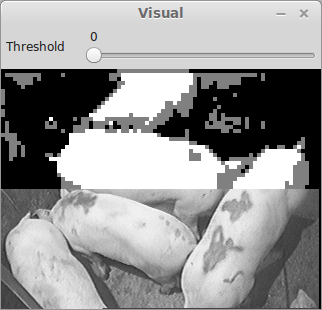
\includegraphics{M1}
  \caption{M1, training data manually clustered based on specifications}
\end{figure}

Using those divisions, we can go through all our testing vectors and find their
nearest neighbor using the Euclidian distance formula, and assign the
corresponding class.

\begin{figure}[H]
  \centering
  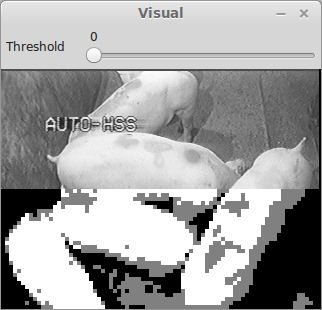
\includegraphics{N1}
  \caption{N1, testing data classified by nearest neighbor vector}
\end{figure}

This give us something a little ugly, and also this result takes a while to
produce. Another way we could estimate this image is to replace the testing data
with the nearest neighbor in the training data.

\begin{figure}[H]
  \centering
  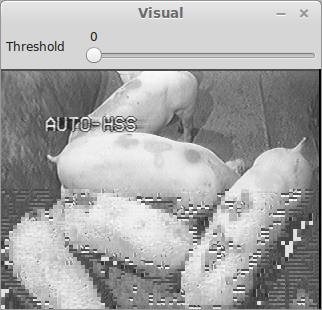
\includegraphics{N2}
  \caption{N2, testing data replaced with nearest neighbor training vector}
\end{figure}

However this gives us results that while quite accurate, are also visually
jarring because of the sharp differences from neighboring vectors. We can smooth
this up a little by replacing the vector with its average value, getting a
smoother, blurred look.

\begin{figure}[H]
  \centering
  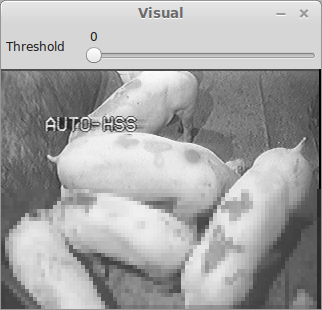
\includegraphics{N3}
  \caption{N3, testing data replaced with nearest neighbor average}
\end{figure}

Even yet still we can try to improve on N1's color accuracy by changing the
colors to the average color of all the vectors in each corresponding class.

\begin{figure}[H]
  \centering
  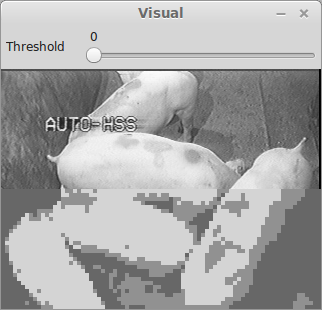
\includegraphics{N4}
  \caption{N4, testing data replaced with nearest neighbor class average}
\end{figure}

Assessing N1 a bit more, we can manually replace the testing vectors like we did
with M1 to prodcue T1 and compute the error value between our nearest neighbor
predicition N1 and the acutal classification T1.

\begin{figure}[H]
  \centering
  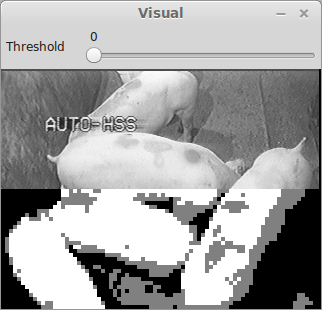
\includegraphics{T1}
  \caption{T1, testing data manually clustered based on specifications}
\end{figure}

\begin{figure}[H]
  \centering
  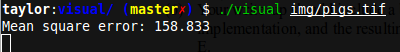
\includegraphics{mse}
  \caption{Mean squared error between N1 and T1}
\end{figure}

We could also try a k-means clustering algorithm to alternatively group the
classes. My result is slightly miscolored, probably because of the ordering of
the initially sampled centers, but the differences between the three classes are
still apparent.

\begin{figure}[H]
  \centering
  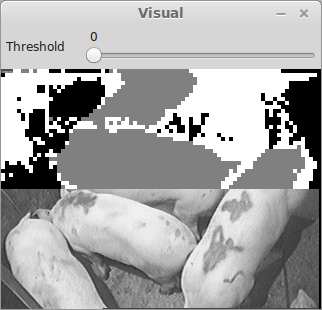
\includegraphics{K1}
  \caption{K1, training data separated by k-means classfication}
\end{figure}

\section{Part B}

Here we examine some motion detection techniques. If we simply take the
difference between two frames, we get the differences overlayed but we can't
really tell what's moving where. We can compensate the difference in motion
between the two frames by using an idea similar to nearest neighbor classifiers
to find the shortest Euclidian distance between $8\times8$ segments of the frames.
The nearest neigbhor is then subtracted from the original image and we get a
better idea of the motion vectors.

\begin{figure}[H]
  \centering
  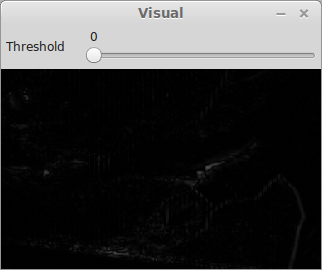
\includegraphics{dumb_ping}
  \caption{The direct difference between the first two frame sets}
\end{figure}

\begin{figure}[H]
  \centering
  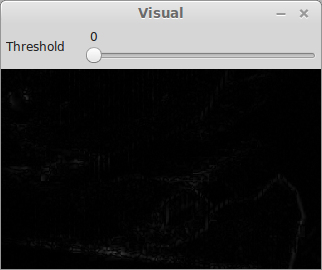
\includegraphics{comp_ping}
  \caption{Compensated difference between the first two frame sets}
\end{figure}

\begin{figure}[H]
  \centering
  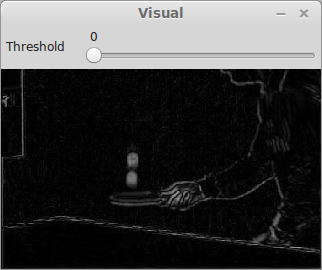
\includegraphics{dumb_pong}
  \caption{Direct difference between the second two frame sets}
\end{figure}

\begin{figure}[H]
  \centering
  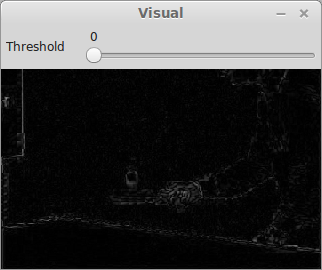
\includegraphics{comp_pong}
  \caption{Compensated difference between the second two frame sets}
\end{figure}

The compensated difference in Figure 12 is especially distinct, as in Figure 11
you can clearly make out 2 distinct balls (their ``shadows''), but the
difference disappears in figure 12 and you can see the motion vectors better.

\section{References}

\begin{enumerate}
\item OpenCV 3.0 Documentation --- http://docs.opencv.org/3.0.0/
\end{enumerate}

\end{document}